\documentclass[9pt]{beamer}
\usepackage{styles/mypreamble}
%~~~~~~~~~~~~~~~~~~~~~~~~~~~~~~~~~~~~~~~~~~~~~~~~~~~~~~~~~~~~~~~~~~~~~~~~~~~~~~
\title{Алгоритмы машинного обучения}
\subtitle{Лекция 6. Рекомендательные системы}
\author{Владимир Кукушкин}
\institute{СПбГЭУ - 23.12.2020}
%~~~~~~~~~~~~~~~~~~~~~~~~~~~~~~~~~~~~~~~~~~~~~~~~~~~~~~~~~~~~~~~~~~~~~~~~~~~~~~

\begin{document}

\titlepage

\section{Постановка задачи}
\begin{frame}{Зачем нужны рекомендательные системы?}
    \begin{itemize}
        \item Побуждать пользователя к совершению дополнительной покупки (рекомендация товаров).
        \item Оставлять пользователя в системе как можно дольше, повышая его удовлетворённость сервисом. В частности, побуждать пользователя продлить подписку (рекомендация контента).
        \item Усиление социального эффекта в соцсетях (рекомендация друзей).
        \item Рекомендации для новых пользователей: быстрое повлечение пользователя в продукт, борьба с оттоком.
    \end{itemize}
\end{frame}

\begin{frame}{Драматичная история}
\begin{itemize}
    \item Netflix prize (2006).
    \item \$1000000 за лучшую рекомендательную систему для видео.
    \item Соревнование проводилось 3 года.
    \item За первый год улучшили изначальное качество на 7\%.
    \item В конце две команды прислали решения, улучшающие текущего лидера на 10\% с одинаковым качеством (в  4 знаке!) с разницей в 20 минут.
    \item Соревнование оказало значительное влияние на развитие рекомендательных систем.
\end{itemize}
\end{frame}

\begin{frame}{Типы рекомендательных систем}
\begin{itemize}
    \item Content-based
    \begin{itemize}
        \item Пользователю рекомендуются объекты, похожие на те, что пользователь уже выбирал.
        \item Похожесть оценивается по признакам объекта.
    \end{itemize}
    \item Коллаборативная фильтрация (collaborative filtration)
    \begin{itemize}
        \item Для рекомендации используется как история самого пользователя, так и других.
    \end{itemize}
\end{itemize}
\end{frame}

\begin{frame}{Какие бывают сигналы (и их проблемы)}
    \begin{itemize}
        \item Явные
        \begin{itemize}
            \item Звёздочки, лайки.
            \item Проблема: субъективность, малое количество голосов.
        \end{itemize}
        \item Неявный
        \begin{itemize}
            \item Покупки (понравилось или нет?)
            \item Время (залип в хороший фильм или включил и ушёл в другую комнату?)
            \item Клик (А что произошло после клика? А если нет клика, это плохо?)
        \end{itemize}
    \end{itemize}
\end{frame}

\begin{frame}{Постановка задачи}
\begin{itemize}
    \item Есть множество пользователей $u\in U$ (users).
    \item Есть множество объектов $i\in I$ (items).
    \item Есть множество событий $(r_{ui}, u, i)\in D$ – действия пользователя $u$ с объектом $i$ и результатом $r_{ui}$.
\end{itemize}

Хотим:
\begin{itemize}
    \item Предсказать предпочтение:
    $$\hat r_{ui} = Predict(u, i) \approx r_{ui},$$
    \item Дать персональные рекомендации:
    $$u\rightarrow (i_1, \ldots,i_K)=Recommend_K(u),$$
    \item Выбрать похожие объекты:
    $$u\rightarrow (i_1, \ldots,i_M)=Similar_M(u).$$ 
\end{itemize}
\end{frame}

\begin{frame}{Постановка задачи}
\begin{center}
    \begin{tabular}{|c|c|c|c|c|c|c|}
    \hline
         & Item 1 & Item 2 & Item 3 & Item 4 & Item 5 & Item 6 \\\hline
    User 1 & 5 & 4 & 5 & & & \\\hline
    User 2 & 4 & & 5 & & & \\\hline
    User 3 & & 3 & 5 & & 4 & \\\hline
    User 4 & & & & 3 & 4 & \\\hline
    User 5 & & & 4 & 2 & 4 & \\\hline
    User 6 & 3 & & & & & 5\\\hline
    \end{tabular}
\end{center}
\end{frame}

\begin{frame}{Постановка задачи}
\begin{center}
    \begin{tabular}{|c|c|c|c|c|c|c|}
    \hline
         & Item 1 & Item 2 & Item 3 & Item 4 & Item 5 & Item 6 \\\hline
    User 1 & 5 & 4 & 5 & \textcolor{red}{?} & \textcolor{red}{?} & \textcolor{red}{?} \\\hline
    User 2 & 4 & \textcolor{red}{?} & 5 & \textcolor{red}{?} & \textcolor{red}{?} & \textcolor{red}{?} \\\hline
    User 3 & \textcolor{red}{?} & 3 & 5 & \textcolor{red}{?} & 4 & \textcolor{red}{?} \\\hline
    User 4 & \textcolor{red}{?} & \textcolor{red}{?} & \textcolor{red}{?} & 3 & 4 & \textcolor{red}{?} \\\hline
    User 5 & \textcolor{red}{?} & \textcolor{red}{?} & 4 & 2 & 4 & \textcolor{red}{?} \\\hline
    User 6 & 3 & \textcolor{red}{?} & \textcolor{red}{?} & \textcolor{red}{?} & \textcolor{red}{?} & 5\\\hline
    \end{tabular}
\end{center}
\end{frame}

\section{Простейшие алгоритмы}

\subsection{Предсказание средним значением}

\begin{frame}{Средние значения}
\begin{itemize}
    \item Почему бы не предсказывать средним значением?
    $$\hat r_{ui} = \frac{\sum\limits_{v\in U_i} r_{vi}}{|U_i|},$$ 
    где $U_i$ – множество пользователей, оценивших объект $i$.
    \item Проблема: у объекта может быть мало оценок или не быть вообще.
    \item Если объект оценил только один пользователь и поставил лайк, то доля лайков будет 100\%.
\end{itemize}
\end{frame}

\begin{frame}{Средние значения - сглаживание малого числа голосов}
    \begin{itemize}
        \item Сглаживание Лапласа для дроби \(\frac{M}{N}\). Выберем некоторые константы \(\alpha, V\):
        $$\frac{M + \alpha}{N + \alpha V}\;\;\underrightarrow{N\rightarrow \infty}\;\;\frac{M}{N}$$
        \item Добавим \(k\) фиктивных голосов со средним значением \(\mu\):
        $$\hat r_{ui} = \frac{\sum\limits_{v\in U_i} r_{vi} + k\mu}{|U_i| + k}$$
    \end{itemize}
\end{frame}

\subsection{Предсказание по доверительному интервалу лайков}

\begin{frame}{Лайки и Бернулли}
\begin{itemize}
    \item Если мы видим, что у объекта 200 лайков и 180 дизлайков, стоит ли его рекомендовать?
    \item Брать просто дельту плохо. Лучше проверить стат.гипотезу.
    \item А ещё лучше оценить вероятность лайка и построить доверительный интервал.
\end{itemize}
\end{frame}

\begin{frame}{Доверительный интервал для лайков}
\begin{itemize}
    \item Количество лайков моделируется биномиальным распределением.
    \item Биномиальное распределение хорошо приближается нормальным.
    \item Если $p$ – вероятность лайка, $M$ – число лайков, $N$ – общее число голосов,  то распределение оценки вероятности:
    $$\hat p = \frac{M}{N} \sim \mathcal{N}\left(\hat p, \frac{\hat p(1-\hat p)}{N}\right).$$
    \item Доверительный интервал уровня $\alpha$:
    $$\left(\hat p - z_{\alpha /2} \sqrt{\hat p(1-\hat p)/N},\;\hat p + z_{\alpha/2}\sqrt{\hat p(1-\hat p)/N}\right),$$
    где $z_{\alpha/2}$ – квантиль нормального распределения.
    \item Рекомендуем по нижней границе.
\end{itemize}
\end{frame}

\subsection{Content-based рекомендации}

\begin{frame}{Рекомендация похожих объектов}
\begin{itemize}
    \item Хотим найти похожие товары по каким-то признакам и при просмотре одного из них рекомендовать другой.
    \item Чем-то похоже на ассоциативные правила, но в АП у нас было условие и следствие (работало в одну сторону). Здесь же именно что хотим найти похожие объекты.
    \item Например: игровая консоль и диски для игр похожи. Если купил консоль, то наверняка купит и диски. Но если купил диски, то не обязательно купит консоль.
    \item Наивный подход: перебрать все пары и посмотреть, как часто объекты $i_0$ и $i_1$ покупают вместе.
    \item Так просто не работает, потому что с высокой вероятностью на месте $i_1$ окажется не похожий на $i_0$ объект, а самый частотный.
\end{itemize}
\end{frame}

\begin{frame}{Метрика похожести объектов}
    \begin{itemize}
        \item Метрика Жаккара:
        $$J(A, B)=\frac{|A\cap B|}{|A\cup B|}=\frac{|A\cap B|}{|A| + |B| - |A\cap B|}.$$
        \item $A$ – множество людей, выбравших объект $i_0$.
        \item $B$ – множество людей, выбравших объект $i_1$.
        \item Чем чаще покупают редкие товары, тем лучше.
        \item Знаменатель защищает от частотных товаров.
    \end{itemize}
    
    \begin{center}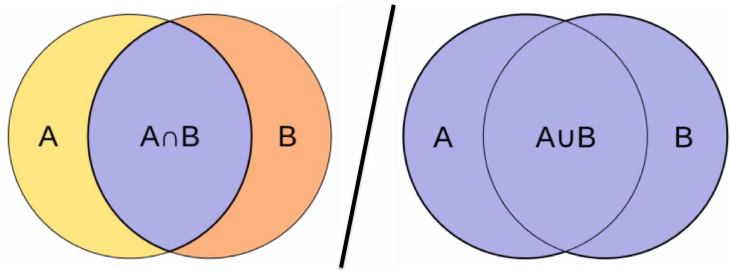
\includegraphics[height=100px]{img/jaccard.png}\end{center}
\end{frame}

\begin{frame}{Технические особенности вычисления метрики Жаккара}
\begin{itemize}
    \item Если вычислять в лоб, то сложность $O(M\cdot M \cdot N)$, где $M$ – количество объектов, $N$ – количество пользователей.
    \item Но нам нужны только те пользователи, выбравшие оба объекта из данной пары.
    \item Инвертированный индекс: будем хранить только те пары, которые купил хотя бы один пользователь. Бежать в цикле будем не по парам срок, а по стоблцам, и только по тем элементам, где есть единички.
\end{itemize}

\begin{center}
\begin{tabular}{p{0.4\textwidth}p{0.4\textwidth}}
     \begin{center}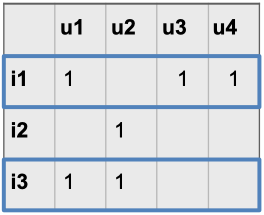
\includegraphics[height=75px]{img/jaccard_inv_index_1.png}\end{center}& 
     \begin{center}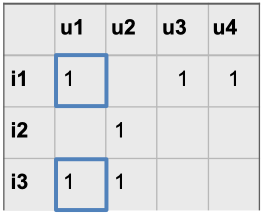
\includegraphics[height=75px]{img/jaccard_inv_index_2.png}\end{center}\\
     Бежать по строкам плохо & Будем бежать по столбцам, по тем товарам, где есть единички \\
\end{tabular}
\end{center}
\end{frame}

\section{Коллаборативная фильтрация (Collaborative filtering)}
\begin{frame}{Идея}
\begin{itemize}
    \item Хотим группировать по похожести и пользователей, и объекты.
    \item Тогда похожим пользователям можно будет рекомендовать похожие объекты.
\end{itemize}
\end{frame}

\framedgraphic{Коллаборативная фильтрация. Пример.}{img/collaboration_filtering_1.png}
\framedgraphic{Коллаборативная фильтрация. Пример.}{img/collaboration_filtering_2.png}
\framedgraphic{Коллаборативная фильтрация. Пример.}{img/collaboration_filtering_3.png}

\subsection{User-based подход}

\begin{frame}{User-based CF}

\begin{itemize}
    \item Начнём с поиска похожих пользователей.
     \item Как можно понимать похожесть объектов/пользователей?
     \item И пользователи, и объекты -- это некоторые векторы. Нужна метрика близости векторов $d$.
     \pause
     \item Корреляция.
     \pause
     \item Косинусное расстояние:
     $$cos(x, y) = \frac{xy}{\|x\|\|y\|}.$$
\end{itemize}
\end{frame}

\begin{frame}{Корреляция оценок}
    \begin{itemize}
        \item Корреляция Пирсона:
        $$\rho(u_1, u_2) = \frac{\sum\limits_{i\in I_{u_1}\cap I_{u_2}} (r_{u_1, i} - \bar r_{u_1}) (r_{u_2, i} - \bar r_{u_2})}{\sqrt{\sum\limits_{i\in I_{u_1}\cap I_{u_2}} (r_{u_1, i} - \bar r_{u_1})^2} {\sqrt{\sum\limits_{i\in I_{u_1}\cap I_{u_2}} (r_{u_2, i} - \bar r_{u_2})^2}}  }$$
        \item Считаем только по общим рейтингам $i\in I_{u_1}\cap I_{u_2}$.
        \item $\bar r_{u_1}, \bar r_{u_2}$ – средняя оценка пользователя (по всем объектам из $I_{u_1}$, $I_{u_2}$ соответственно).
    \end{itemize}
\end{frame}

\begin{frame}{Пример}
\begin{center}
\begin{tabular}{p{0.4\textwidth}p{0.6\textwidth}}
     \begin{center}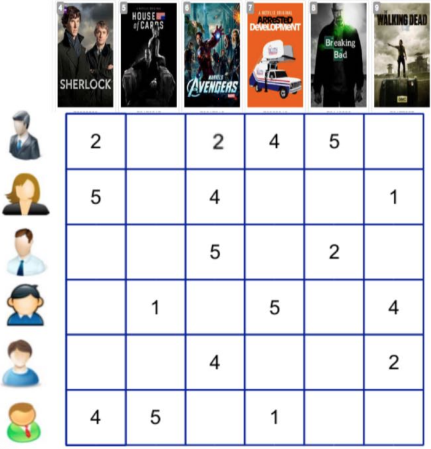
\includegraphics[height=150px]{img/collaborative_filtering_correlation.png}\end{center}&
     \begin{itemize}
        \item Определим, кто похож на пятого пользователя.
        \pause
        \item С первым и шестым -- NA.
        \item $\d(u_5, u_2) = \frac{(4-3)(4-3.33) + (2-3)(1-3.33)}{\sqrt{(4-3)^2 + (2-3)^2} \cdot \sqrt{(4-3.33)^2 + (1-3.33)^2}} \approx 0.87$.
        \item $\rho(u_5, u_2) = \frac{(4-3)(5-3.5)}{\sqrt{(4-3)^2} \cdot \sqrt{(5-3.5)^2}} = 1$.
        \item $\rho(u_5, u_2) = \frac{(2-3)(4-3.33)}{\sqrt{(2-3)^2} \cdot \sqrt{(4-3.33)^2}} = -1$.
     \end{itemize}
\end{tabular}
\end{center}
\end{frame}

\begin{frame}{Корреляция оценок. Сглаживание.}
\begin{itemize}
    \item Нужен какой-то штраф за маленькие пересечения.
    \item Если одна общая оценка, то корреляция всегда будет $\pm 1$.
    $$d(u_1, u_2) = c\cdot \frac{\sum\limits_{i\in I_{u_1}\cap I_{u_2}} (r_{u_1, i} - \bar r_{u_1}) (r_{u_2, i} - \bar r_{u_2})}{\sqrt{\sum\limits_{i\in I_{u_1}\cap I_{u_2}} (r_{u_1, i} - \bar r_{u_1})^2} {\sqrt{\sum\limits_{i\in I_{u_1}\cap I_{u_2}} (r_{u_2, i} - \bar r_{u_2})^2}}  },$$
где \( c = \min\left(\frac{|I_{u_1}\cap I_{u_2}|}{50}, 1\right)\).
    \item А можно считать доверительный интервал для корреляции.
    \item А ещё нужно выкидывать пользователей с одинаковыми оценками. (Почему?)
\end{itemize}
\end{frame}

\begin{frame}{Оценки похожих пользователей}
    \begin{itemize}
        \item Можно предположить, что у похожих пользователей будут похожие оценки.
        \item Тогда чтобы предсказать оценку пользователя $u$ товару $i$ можно взвешенную среднюю оценку его соседей $NN(u)$ для товара $i$ пропорционально расстоянию до соответствующего пользователя:
        $$\hat r_{ui}=\frac{\sum\limits_{v\in NN(u)}d_{uv} \cdot r_{vi}}{\sum\limits_{v\in NN(U)} d_{uv}}.$$
        \item В таком виде пользователи, которые любят ставить завышенные или заниженные оценки всё испортят.
        \item Нужно стандартизировать все $r_{vi}$.
    \end{itemize}
\end{frame}

\begin{frame}{Оценки похожих пользователей. Стандартизация оценок.}
    \begin{itemize}
        \item Итого:
        $$\hat r_{ui}=\bar r_u + \sigma_u\frac{\sum\limits_{v\in NN(U)}d_{uv}(r_{vi} - \bar r_v)/\sigma_v}{\sum\limits_{v\in NN(u)} d_{uv}}.$$
        \item Суммируем только по ближайшим соседям $NN(u)$, ставившим оценку объекту $i$.
        \item Суммируем стандартизированные оценки $(r_{vi}-\bar r_v)/\sigma_v$ ($\bar r_v$ и $\sigma_v$ считаем по всем оценкам пользователя $v$ в датасете).
        \item Взвешиваем по относительной похожести $\frac{d_{uv}}{\sum_{v\in U_i}d_{uv}}$
        \item Домножаем на $\sigma_u$, чтобы перейти обратно к "единицам измерения"\; пользователя $u$.
        \item Таким образом, второе слагаемое в формуле задаёт ожидаемое отклонение от средней оценки пользователя $u$. Значит, остаётся только добавить это среднее $\bar r_u$.
    \end{itemize}
\end{frame}

\begin{frame}{Проблемы user-based рекомендаций}
\begin{itemize}
    \item У нас по-прежнему сильно разреженная матрица.
    \item Все оценки получаются сильно приближёнными и близкими к средним значениям.
    \item Оценки меняются быстро, и каждая новая оценка будет давать сильное изменение. Возможности пересчитывать предсказания быстро ограничены.
\end{itemize}
\end{frame}

\begin{frame}{Проблемы user-based рекомендаций}
\begin{itemize}
    \item Пусть есть 1000 пользователей, 100 объектов и 10000 оценок равномерно распределены по матрице.
    \item Вероятность того, что в ячейке не пусто: 10\%.
    \item Сколько в среднем объектов будет в пересечении у двух случайных пользователей?
    \pause
    \item Ответ: 1. Вероятность, что второй оценит хотя бы один из 10 объектов первого, равна 0.1. Но второй в среднем оценивает 10 объектов. Значит, вместе в среднем они оценят $10\cdot 0.1 = 1$ объект.
    \item А сколько будет общих пользователей у двух случайных объектов?
    \pause
    \item Ответ: $100 \cdot 0.1 = 10$.
    \item Вывод: перейти от user-based к item-based.
\end{itemize}
\end{frame}

\subsection{Item-based подход}

\begin{frame}{Item-based рекомендации}
    \begin{itemize}
        \item Всё почти же самое, что и в user-based рекомендациях, только теперь теперь смотрим на похожесть объектов.
        \item В качестве метрики похожести объектов обычно берут косинусную меру:
        $$d(i, j) = \frac{ij}{||i||\cdot||j||}.$$
        \item Но тут тоже есть изъяны. Пусть рейтинги объектов $i_1, i_2, i_3$ (1, 1), (2, 2), (5, 5).
        \item Тогда $d(i_1, i_2) = d(i_2, i_3) = d(i_1, i_3) = 1$.
        \item Косинусы одинаковые, но смысл оценок разный.
    \end{itemize}
\end{frame}


\begin{frame}{Item-based рекомендации. Adjusted cosine similarity.}
    \begin{itemize}
        \item В формуле косинусного расстояния центрируем векторы оценок пользователей:
        $$d(i, j) = \frac{\sum\limits_{u\in U_{i}\cap U_{j}} (r_{u, i} - \bar r_{u}) (r_{u, j} - \bar r_{u})}{\sqrt{\sum\limits_{u\in U_i\cap U_j} (r_{u, i} - \bar r_u)^2} {\sqrt{\sum\limits_{u\in U_i\cap U_j} (r_{u, j} - \bar r_u)^2}}  }.$$
        \item Вопрос: чем отличается от корреляции?
        \pause
        \item Ответ: В корреляции бы мы вычитали $\bar r_i$ и $\bar r_j$.
    \end{itemize}
\end{frame}

\begin{frame}{Плюсы, минусы, подводные камни item-based подхода}
\begin{itemize}
    \item Более точный, чем user-based, потому что больше информации в пересечении $U_i\cap U_j$.
    \item Как следствие, более устойчив к новым оценкам.
    \item На практике это означает, что можно пересчитывать похожести всех пар условно раз в сутки (не слишком часто).
\end{itemize}
\end{frame}

\begin{frame}{Выводы по коллаборативной фильтрации}
\begin{itemize}
    \item Плюсы:
    \begin{itemize}
        \item Неплохой метод для начала.
        \item Работает лучше, чем content-based.
    \end{itemize}
    \item Минусы.
    \begin{itemize}
        \item Пользователи должны оценивать одинаковые товары.
        \item Плохо работает, когда матрица разрежена.
        \item Проблема холодного старта: не знаем, что делать с новым объектом или новым пользователем.
    \end{itemize}
\end{itemize}
\end{frame}

\section{SVD-based методы}



\begin{frame}[allowframebreaks]
    \frametitle{Литература}
    \bibliographystyle{unsrt}
    \nocite{rec_systems_cs_center}
    \nocite{rec_systems_habr}
    \bibliography{references.bib}
\end{frame}

\end{document}